\section{Atomic Bonded Cross-chain Debt}
\label{sec:abcd}

\newfateme{To make the ABCD primitive, we have to consider two problems. First, the Alice defaults and anti-cheat transactions have inputs from both sides. Second, the redemption and Bob's principal deposition transactions should not have any outputs since their inputs are dynamically determined through the protocol and after creation when we did not have the hashes. To solve either problem, we are going to remove the exercise lock stage from the procedure. The main goal of this stage was to inhibit Bob's cheating. To remove this stage, we need to eliminate the cheating incentive by a different manner. The functionality of the delay keeper stage also needs to be noticed. We have to design the protocol in such a way that when Alice fulfills her redemption, Bob has the minimum needed time to reveal the} \new{\keyone key.} 
% Since the Alice's time's up transaction in the ABD primitive needs to be shared in both Alice's and Bob's stages, this form of bond can not be used across different blockchains. To solve the problem of interoperability for the atomic bond\new{,} we have redesigned our model using check-sequence-verify\footnote{The up-code CHECKSEQVERIFY}.


% In this section, we first build an intermediary component that has the same functionality as ABD. After that, we introduce \new{ABCD} that can be actually used between different blockchains.


% Using the check-sequence-verify, the minimum amount of coins for the determinator transaction and the delay keeper stage are removed from the component.

\begin{figure}
  \centering
  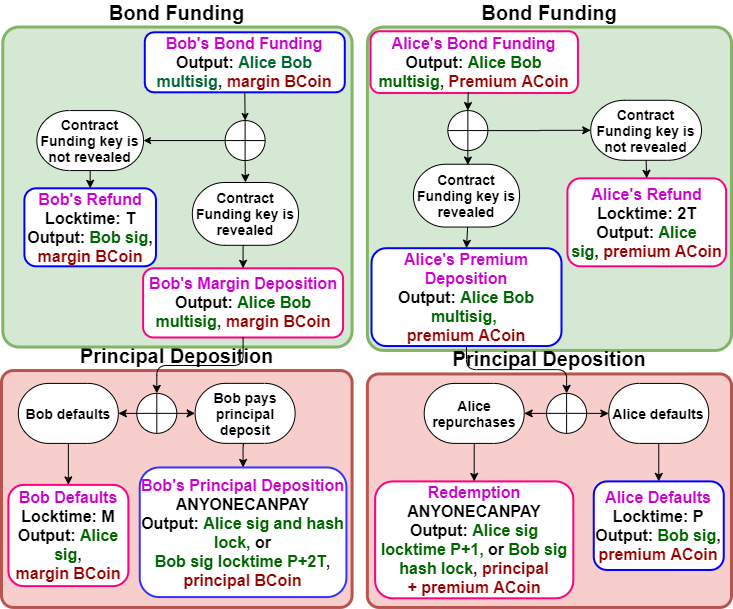
\includegraphics[width=\linewidth]{figures/ABCDfateme.png}
 \caption{The ABCD component. On each transaction, signatures, output amount and locktimes are specified. All outputs are in the same coin. Pink-bordered transactions are broadcast by Alice and blue-bordered ones by Bob. For locktimes, \newfateme{Unix timestamp} is used. Upper transactions are broadcast earlier than the lower ones. If there is a line between two transactions, then the source transaction is considered to be an input of the destination transaction.}
  \Description{An atomic bonded debt}
  \label{fig:non-collat-bond}
\end{figure}

The first ABCD component is demonstrated in Fig\new{.}~\ref{fig:non-collat-bond}. To present this type of ABCD we use \newfateme{Unix time} as the locktime parameter. However, the block height can also be used. The procedure is discussed below:

\begin{itemize}
    \item \textbf{Bond Funding}: Alice's funding includes premium and Bob's includes margin. \newfateme{The number $T$ is the minimum time needed for a transaction to be confirmed.} \newfateme{Here, the premium will not be directly sent to Bob after revealing the} \new{\Aone} \newfateme{key and will be locked in the Alice's premium deposition transaction.}
    
    \item \textbf{Principal Deposition}: 
        After issuing the bond, similar to the general model, each party has to deposit their principal within a specified time interval: Bob $M$ locktime and Alice $P$ ($P > M$). \newfateme{Both} Bob's principal deposition  \new{and} Alice's \new{redemption} transactions have sighash type of anyone-can-pay since only on of their inputs is determined at the time of creating the transaction. Bob can behave in one of the two following ways:
    \begin{itemize}
        \item He defaults, then Alice takes his margin by broadcasting the Bob defaults transaction.
        \item He deposits the principal, \newfateme{and waits for action of Alice.}
    \end{itemize}
    % \item \textbf{Exercise Lock}: If Bob deposits his principal before the locktime, Alice has time before a $P$ locktime expires to \new{repurchase} her \new{bond}. As mentioned earlier, the \new{redemption} transaction has sighash type of no-input. The \new{``}checkseq 1" in the anti-cheat transaction, forces this transaction to have a minimum block distance of 1 from its parent i.e. the anti-cheat transaction can only be mined in a block with a higher block height than the block which Alice's \new{redemption} transaction is in, hence Bob has enough time to reveal the \keyone key. Note that the 1 block height difference may have to vary in different blockchains. For example in bitcoin, the minimum block height needed to elapse for the transactions to be confirmed is 6 blocks. Thus, we have to use \new{``}checkseq 6" in bitcoin. However, in this context, we assume the general case of 1 block.
    
    After Bob's principal deposition, there are two possible scenarios based on decision of Alice: 
    \begin{itemize}
        \item Alice succeeds to \new{repurchase}. Bob reveals the \keyone key. \newfateme{Finally, Alice can take her bond and the premium will be sent to Bob.}% The result is similar to the original ABD. 
        
        \item Alice does not broadcast the \new{redemption} transaction. Therefore, Bob avoids exposing the \keyone key and his principal is sent back to himself. To achieve this, Bob gives Alice \newfateme{$P$} locktime to convince him to reveal the \keyone key and if this deadline is passed, he will broadcast the Alice defaults transaction \newfateme{which gives him the premium as well.}
        
        \item Alice fulfills her \new{redemption} transaction but Bob does not reveal the \keyone key. In this case, Alice can take back her principal and premium.
        % broadcast the anti-cheat transaction to get her principal and a portion of Bob's principal as the punishment. 
        % Note that, since the anti-cheat transaction has a locktime of $P + 1$ and a checkseq of 1 and the Alice's defaults transaction has a locktime of $P + 1$, Alice has to broadcast her \new{redemption transaction} before $P$. Otherwise, she would not have enough time to broadcast the anti-cheat transaction in the case of Bob cheating. In other words, if the Alice's \new{redemption} transaction is mined in a block of at least $P + 1$ height and Bob does not reveal \keyone key, she can not get the anti-cheat transaction mined before block $P + 2$. Therefore, Bob can broadcast the Alice defaults in the $P + 1$th block and avoid giving her the capital.
    \end{itemize}
    \newfateme{Note that Alice has only $P$ locktime to fulfill her redemption transaction, and to get the redemption's output, she has to wait until $P+T$ locktime. Thus, Bob has the minimum required time to reveal the} \new{\keyone} \newfateme{key and receive his payback. Also, Alice can not deposit the redemption transaction at the very last moments and spend the output of redemption. Hence, the output script of the redemption transaction achieves the purpose of the delay keeper stage in the previous section.}
\end{itemize}

\newfateme{So far, we have made the first ABCD primitive. However, one last important issue is remaining. In this form of ABCD, Bob's only inhibitor from cheating is the amount of premium. Since the cryptocurrencies market faces significant fluctuations periodically over time, the value of the BCoin principal may rise higher than the payback plus premium value in ACoin. This rise incentivizes Bob to ignore the premium and get back his principal.}
% The reason which prevents the intermediary ABD component to be used in a cross-chain environment is that the anti-cheat transaction has inputs from both Alice's and Bob's sides. 
To overcome this issue, before exploiting any bond contract, Bob, who is considered to be an exchange or somebody who has a reasonable amount of assets in different blockchains, can deposit some assets as a bond guarantee in any desired chain. Then, \newfateme{we can adjust Bob's guarantee based on the current fluctuation ratio of the market to reduce the probability of Bob's undesired decision. }
% Bob can offer his customers a cross-chain bond service that accepts his payback \new{on} the other chain. 
This modification can be seen in Fig.\ref{fig:cross-chain-non-collat-bond}. \newfateme{In this figure, we use Unix timestamp for locktimes and consider the maximum time among all of the involved blockchains since the number of blocks needed for confirmation is different in different blockchains. We can also use the block height.} 

\begin{figure}[]
  \centering
  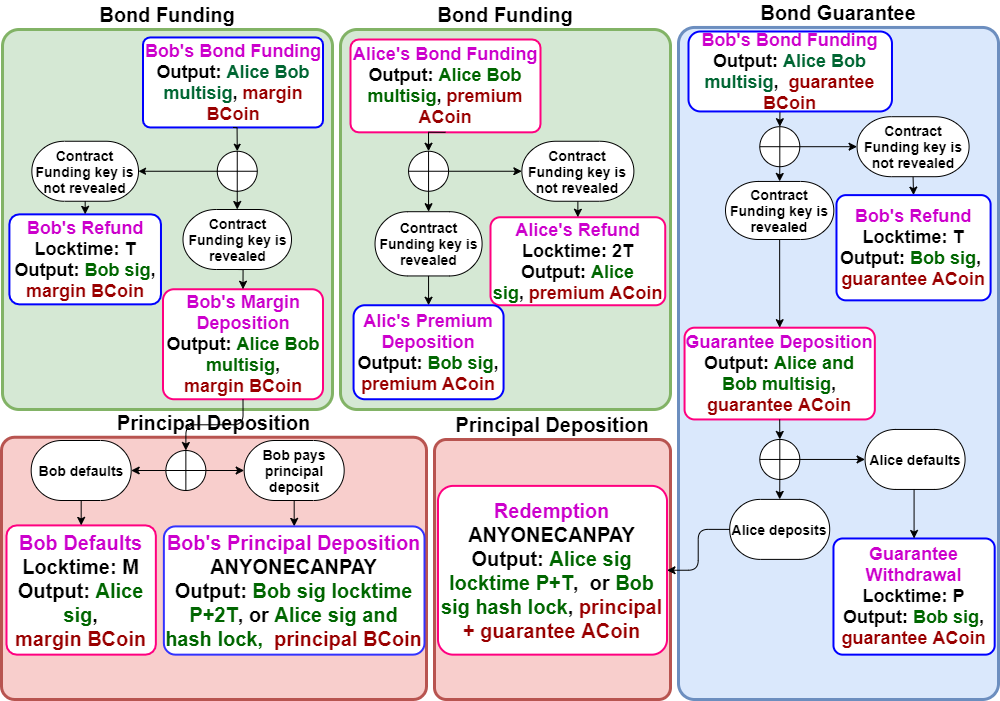
\includegraphics[width=\linewidth]{figures/ABCDfateme2.png}
  \caption{The ABCD across different chains. On each transaction, signatures, output amount and locktimes are specified. Bob's depositions are in BCoin and Alice's in ACoin. Pink-bordered transactions are broadcast by Alice and blue-bordered ones by Bob. For locktimes, Unix timestamp is used. Upper transactions are broadcast earlier than the lower ones. If there is a line between two transaction, then the source transactions is considered to be an input of the destination transaction. \newfateme{To observe an implementation of this structure where the bond is going to be used in an atomic swap, see} \cite{abcd-ref}.}
  \Description{A cross-chain atomic bonded debt.}
  \label{fig:cross-chain-non-collat-bond}
\end{figure}

The difference between the \newfateme{newly designed ABCD component and the previous ABCD} primitive is the addition of the guarantee withdrawal transaction \newfateme{and its related funding transactios}. Whether Alice defaults or the bond is successfully \newfateme{repurchased}, Bob has to broadcast the \new{\emph{guarantee withdrawal}} transaction. \newfateme{Additionally, in the case of not revealing the} \new{\Aone} \newfateme{key, Bob can take his guarantee back. Also, the premium will be sent directly to Bob in all possible scenarios at the beginning of the protocol.} Other parts are the same in both procedures.


% The details of the ABCD is same as the intermediary ABD except for 